% !TEX spellcheck = en_US

% ======================================= V
% (NC) 2019 Haluk Bingol
% github.com/halukbingol/LaTeX-Templates
%
% Licensees may copy, distribute, display, and perform the work and make derivative works 
% and remixes based on it only for non-commercial purposes. 
% ======================================= A




\documentclass[drafts]{beamer}
\usepackage[utf8]{inputenc}

%\usetheme{Montpellier}
\usetheme{Dresden}
\usepackage{beamerthemesplit}

\usepackage{graphicx,epstopdf}
\usepackage{color}
\usepackage{subfigure}


% =======================================
% HB References
\newcommand{\hbReference}[1]{\textcolor{blue}{{\scriptsize [#1]}}}
\newcommand{\hbRemark}[1]{\textcolor{orange}{#1}}

% separator
\newcommand{\hbSection}[2]{
	\section{{#1}} 
	\begin{frame}
		\hbRemark{{\center{\Huge {#1}}}}\\
		{#2}
	\end{frame}
}
\newcommand{\hbSeparator}[2]{
	\begin{frame}
		\hbRemark{{\center{\Huge {#1}}}}\\
		{#2}
	\end{frame}
}


% HB PageNumber/TotalPages
\newcommand*\oldmacro{}%
\let\oldmacro\insertshorttitle%
\renewcommand*\insertshorttitle{%
	\oldmacro\hfill%
	\insertframenumber\,/\,\inserttotalframenumber%
}

% =======================================


% =======================================
\title
	[Running title]
	{
		The Title Here
	}
\author
	[Bingol]
	{
		Haluk O. Bingol
	}
\institute{
	Dept. of Computer Engineering\\
	Bogazici University\\
	Istanbul, Turkey
}
\date{ 
%	\today
	Meeting, City, Feb. 23, 2017
}


%\setbeamertemplate{footline}
%{%
%\insertpagenumber
%}



% =======================================
\begin{document}




% ===================
\frame{\titlepage}



% ===================
\begin{frame}[t]\frametitle{Outline}
	\begin{columns}[T]
	\column{0.6\textwidth}
		\hspace{0.5cm}
		\tableofcontents
	\column{0.5\textwidth}
		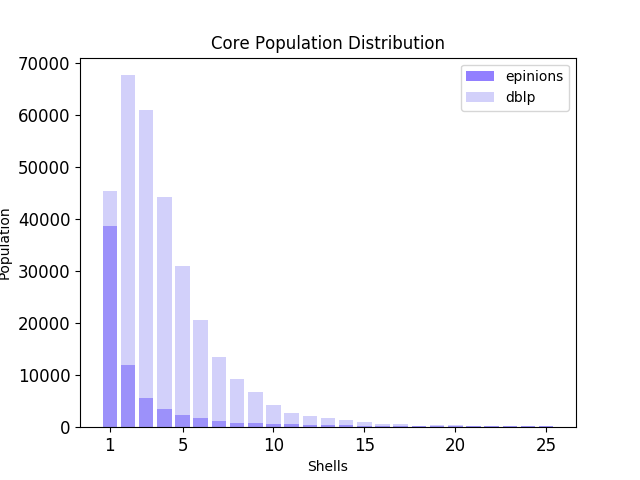
\includegraphics[width=\textwidth]
			{Fig-B}\\
		\hbReference{\href
			{https://en.wikipedia.org/wiki/Blind_men_and_an_elephant}
			{https://en.wikipedia.org/wiki/\\
			Blind\_men\_and\_an\_elephant}}
	\end{columns}
\end{frame}




% =======================================
\hbSection{Section A}




% =======================================
\begin{frame}[t]
{Aaaaa}
\framesubtitle{A2222}
	\begin{alertblock}
		{Bbbbb}
		\begin{itemize}
			\item 
			Ccccc \hbRemark{dddd} ccccc
			\item 
			Eeee
		\end{itemize}
	\end{alertblock}
\end{frame}




% =======================================
\hbSection{Section B}
	{\vspace*{1cm}
		\hbReference{
			Cetin and Bingol, 
			The dose of the threat makes the resistance for cooperation,
			\emph{ Advances in Complex Systems} (accepted), 
			2017.
			\href
				{https://arxiv.org/abs/1605.08682}
				{arXiv:1605.08682}
		}
	}




% =======================================
\begin{frame}[t]
	{A sample of overlay slides}
	\framesubtitle{Single slide definition creates two slides}
	\vspace*{-0.5cm}
\begin{columns}[t]
\column{0.5\textwidth}
	\begin{itemize}
		\item 
		 \hbRemark{$N$}: Number of agents 
		\item
		Aaaaa $N \choose 2$ pairs
	\end{itemize}
\pause % +++++
\column{0.5\textwidth}
	\begin{block}
		{Agent \hbRemark{$i$}}
		\begin{itemize}
			\item 
			\hbRemark{$M_{i}$}: Memory size of $i$
			\item 
			$\hbRemark{\mu_{i}} = \frac{M_{i}}{N}$: Memory ratio of $i$
			\item 
			\hbRemark{$\rho_{i}$}: Probability of defection of $i$
		\end{itemize}
	\end{block}
\end{columns}
\end{frame}




% =======================================
\begin{frame}[t]
	{2-column follows 1-colum}
	\framesubtitle{Aaaaa}
\begin{columns}[t]
%
\column{0.5\textwidth}
	\begin{figure}
		\vspace*{-1cm}
		\includegraphics[width=0.6\columnwidth]%
			{fig-A.pdf}
	\end{figure}
%
\column{0.5\textwidth}
	Right column\\
	Agent \hbRemark{$i$}
	\begin{itemize}
		\item 
		\hbRemark{$M_{i}$}: Memory size of $i$
		\item 
		$\hbRemark{\mu_{i}} = \frac{M_{i}}{N}$: Memory ratio of $i$
	\end{itemize}
\end{columns}
%

	1-column here
	Note that: $\mu_{i}, \rho_{i} \in [ 0, 1]$
	\begin{itemize}
		\item
		Visualization of $i$ as $(\mu_{i}, \rho_{i})$
		\item
		Visualization of population as  as $(\overline{\mu}, \overline{\rho})$
		\begin{itemize}
			\item 
			$\hbRemark{\overline{\mu}} = \frac{1}{N} \sum^N_{i=1} \mu_i$
		\end{itemize}
	\end{itemize}
\end{frame}




% =======================================
\subsection{Subsection B}




% =======================================
\hbSeparator{Simulations}




% =======================================
\begin{frame}[t]
\frametitle{Ttttt ttttt}
\framesubtitle{T2222 2222}
\begin{columns}[t]
%
\column{.8\textwidth}
	\vspace*{-0.3cm}
	\begin{alertblock}{Aaaaa}
		\begin{itemize}
			%
			\item
			\hbRemark{Bbbbb} cccc cccc
			\begin{itemize}
				\item 
				dddd 
				\item
				eeee
			\end{itemize}
			%
			\item
			\hbRemark{Fffff} gggg
			\begin{itemize}
				\item 
				hhhh 
				\item
				jjjj
			\end{itemize}
		\end{itemize}
	\end{alertblock}
	Kkkk
%
\column{.3\textwidth}
	\vspace*{-0.2cm}
%	\includegraphics[width=\columnwidth]%
%		{Figures/TheDose/p5p3p1n0/p5p3p1p0traje.pdf}\\
	\includegraphics[width=\columnwidth]%
		{fig-A.pdf}
\end{columns}
\end{frame}




% =======================================
\begin{frame}[t]
{Take home message}
	\begin{itemize}
		\item 
		Aaaaa
		\item 
		Bbbbb
		\begin{itemize}
			\item
			B-ccccc
			\item
			B-dddd
		\end{itemize}
		\item
		Eeeee
	\end{itemize}
\end{frame}



% =======================================
\section{References}




% =======================================
%; References
\begin{frame}[t]
{References}
	\begin{scriptsize}
		\vspace*{-0.35cm}
		\begin{block}{\hbRemark{Threat Game}}
			\begin{itemize}
				\vspace*{-0.2cm}
				\item
				Cetin and Bingol,
				\textbf{The Dose of the Threat Makes the 
				Resistance for Cooperation},
				\emph{ Advances in Complex Systems}, (accepted)
				2017.\\
				\href
					{https://arxiv.org/abs/1605.08682}
					{arXiv:1605.08682}
			\end{itemize}
		\end{block}
		\vspace*{-0.35cm}
		\begin{block}{Attention Game}
			\begin{itemize}
				\vspace*{-0.2cm}
				\item
				Cetin and Bingol, 
				\textbf{Iterated Prisoners Dilemma with limited attention}, 
				\emph{Condensed Matter Physics}, 
				\textbf{17}, 33001, 
				2014.\\
				DOI:10.5488/CMP.17.33001
				\href
					{https://arxiv.org/abs/1405.0343}
					{arXiv:1405.0343}
			\end{itemize}
		\end{block}
		\vspace*{-0.35cm}
		\begin{block}{Fame Game}
			\begin{itemize}
				\vspace*{-0.2cm}
				\item
				Cetin and Bingol,  
				\textbf{Attention competition with advertisement}, 
				\emph{Phys. Rev. E}, \textbf{90}, 032801,
				2014.\\
				DOI: 10.1103/PhysRevE.90.032801
				\href
					{https://arxiv.org/abs/1211.0156}
					{arXiv:1211.0156}
				\item
				Bingol,
				\textbf{Fame emerges as a result of small memory},
				\emph{Phys. Rev. E}, \textbf{77}, 036118,
				2008.\\
				DOI: 10.1103/PhysRevE.77.036118
				\href
					{https://arxiv.org/abs/nlin/0609033}
					{arXiv:nlin/0609033}
			\end{itemize}
		\end{block}
	\end{scriptsize}
\end{frame}


\end{document}
